\documentclass[conference]{IEEEtran}

\usepackage{amsmath,amssymb}
\usepackage{booktabs}
\usepackage{cite}
\usepackage{graphicx}
\usepackage{hyperref}
\usepackage{listings}
\usepackage{xcolor}

\definecolor{dagentsSoft}{HTML}{F3F6FA}
\definecolor{dagentsLine}{HTML}{CBD5E1}
\definecolor{dagentsCode}{HTML}{152238}

\lstdefinestyle{dagents}{
  basicstyle=\ttfamily\footnotesize\color{dagentsCode},
  breaklines=true,
  columns=fullflexible,
  frame=single,
  rulecolor=\color{dagentsLine},
  backgroundcolor=\color{dagentsSoft}
}

\title{Final Report: Dagents, a Functional Planning Framework for Data Agents}

\author{
\IEEEauthorblockN{Pradyun Devarakonda \quad Dheeraj Rajanala}
\IEEEauthorblockA{
Programming Languages Course Project\\
IMT2022525, IMT2022093}
}

\begin{document}
\maketitle

\begin{abstract}
Dagents is a reusable framework for data computation agents. It supports
source-level computation through Local Monitoring Agents (LMA), multi-source
coordination through a Global Monitoring Agent (GMA), service APIs for pipeline
and workload execution, and OCaml modules for functional planning. The main
programming languages idea is simple: keep stateful runtime work in services,
but move validation, routing, planning, and manifest generation into typed,
deterministic functional modules. This report describes the final state of the
project, the OCaml functional programming layer, the runtime services, and the
NL2SQL quick demo app that uses Dagents end to end.
\end{abstract}

\begin{IEEEkeywords}
functional programming, OCaml, data agents, ML orchestration, NL2SQL,
pipeline planning, Kubernetes
\end{IEEEkeywords}

\section{Introduction}

Many data and ML systems need the same repeated tasks: profile a source,
validate a schema, check data quality, choose a model, run a workflow, and
deploy the required workload. These tasks often become scattered across
services as conditional code. That makes the system harder to test and harder
to explain.

Dagents solves this by separating planning from execution. Runtime services
handle APIs, storage, model execution, and deployment. The OCaml layer handles
pure planning work. It accepts typed or JSON-backed inputs and returns explicit
plans, reports, routes, or manifests.

The project also includes an NL2SQL quick demo. The demo takes a database
schema and a natural language question, generates SQL, and shows a Dagents
trace. This trace proves that the app is not a standalone wrapper. It uses
Dagents planners, core-service, pipeline-service, model-service, LMA, and GMA.

\section{Project Goal}

The goal was to build a working data-agent framework and use functional
programming where it fits naturally. The OCaml code is not a general-purpose
compiler. In this project, words such as compiler and planner mean a
domain-specific translator from one Dagents contract to another.

The main goals were:

\begin{itemize}
  \item support one local computation agent per source;
  \item support one global agent for multi-source computation;
  \item provide reusable service APIs for pipelines, model jobs, topology, and
  workload generation;
  \item use OCaml for typed planning, validation, routing, and rendering;
  \item expose OCaml through a JSON process boundary using \texttt{dagentsc};
  \item show app-level usage through the NL2SQL quick demo.
\end{itemize}

\section{Project Context}

Dagents uses two agent levels. The local agent is called LMA in the codebase.
It can also be explained as a source-level computation agent. The GMA is the
global agent. It registers local agents, receives source outputs, and prepares
aggregate or multi-source computation.

\begin{figure*}[t]
\centering
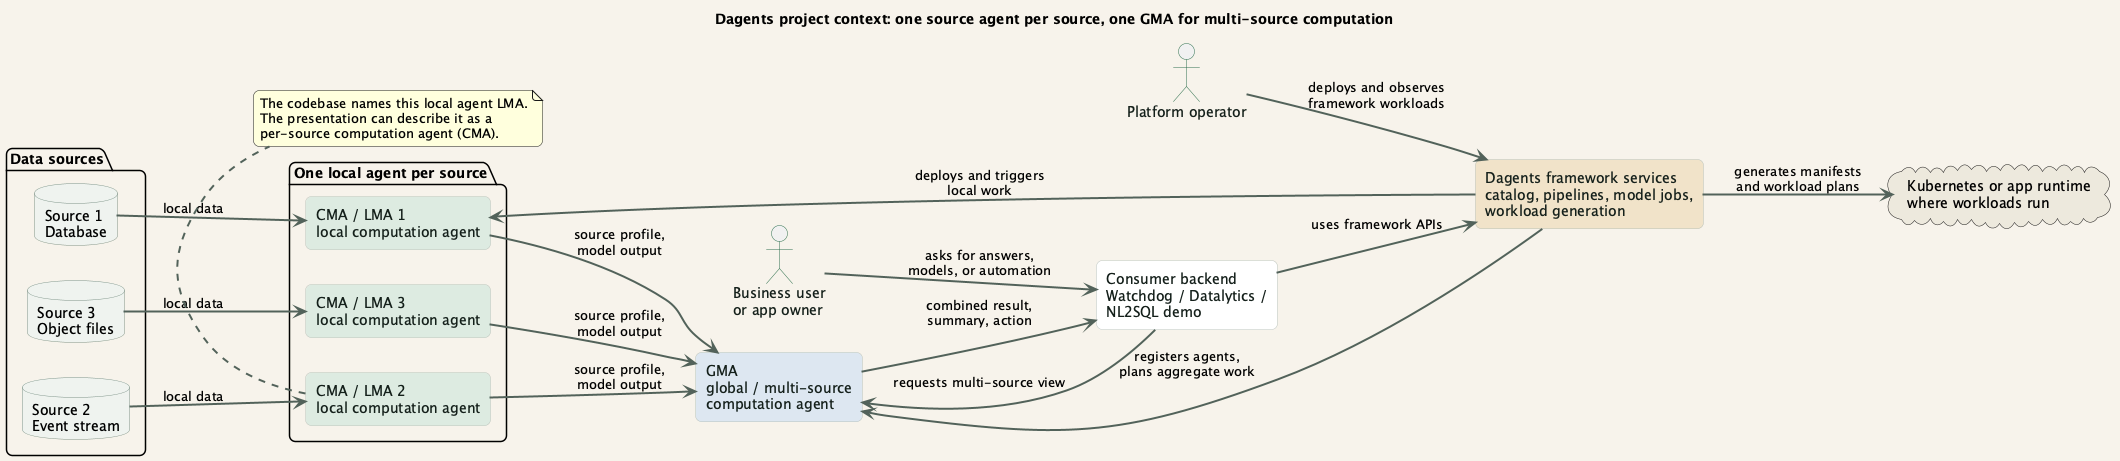
\includegraphics[width=\textwidth]{../presentation/puml/dagents_project_context.png}
\caption{Project context: source-level agents feed a global multi-source agent.}
\label{fig:context}
\end{figure*}

Figure~\ref{fig:context} shows the non-technical view. A product backend, such
as Watchdog, Datalytics, or the NL2SQL demo, uses Dagents services. Each data
source can have its own LMA. The GMA combines local outputs and coordinates
multi-source work.

\section{High-Level Architecture}

The full project is a polyglot system. Python is used for FastAPI services,
ML-related work, and integration. Spring Boot services are present for control
and core-service variants. OCaml is used for the functional planner layer.

\begin{figure*}[t]
\centering
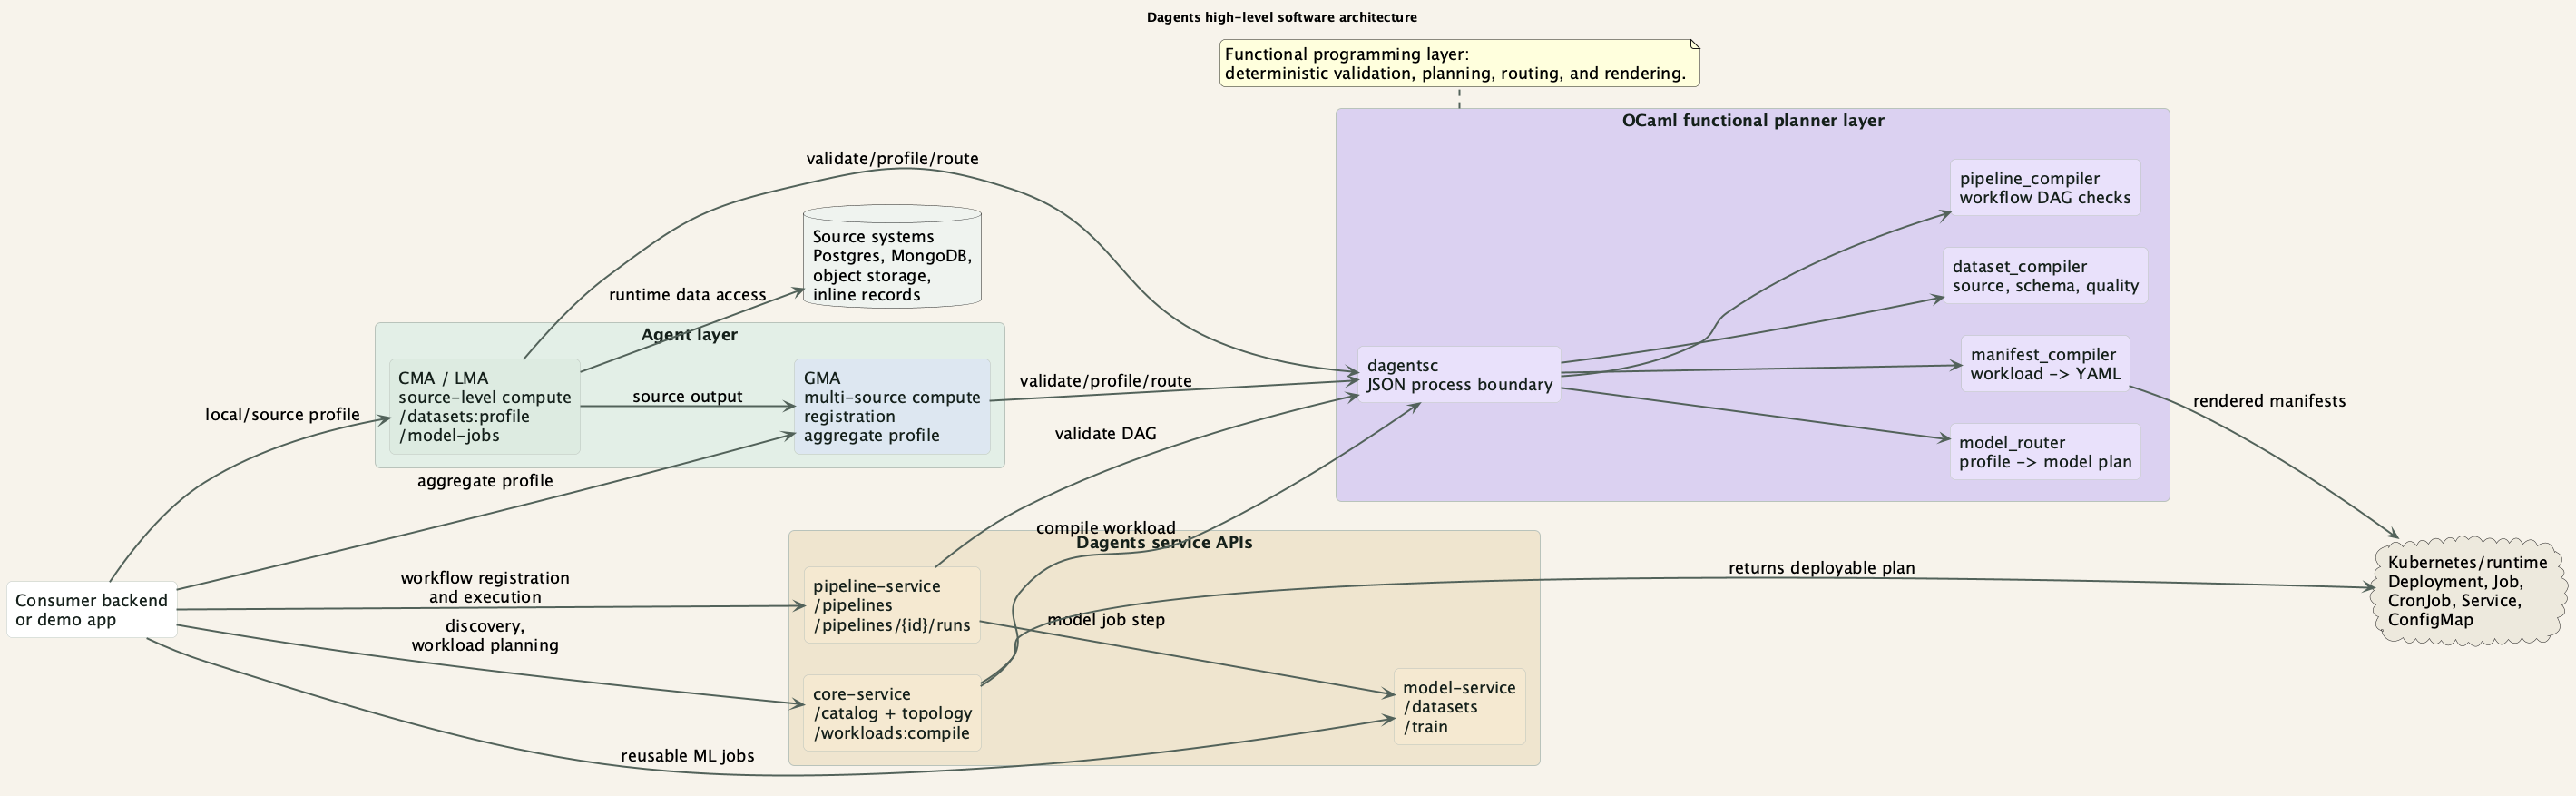
\includegraphics[width=\textwidth]{../presentation/puml/dagents_software_architecture.png}
\caption{High-level software architecture of Dagents.}
\label{fig:software}
\end{figure*}

The main runtime parts are:

\begin{itemize}
  \item \textbf{core-service}: health, service catalog, topology, and workload
  plan generation.
  \item \textbf{pipeline-service}: JSON workflow registration and execution.
  \item \textbf{model-service}: dataset catalog, model training, model jobs,
  and source checks.
  \item \textbf{LMA}: source-level profiling and model execution.
  \item \textbf{GMA}: registration, heartbeat, deployment sync, aggregate
  profiling, and aggregate model execution.
  \item \textbf{OCaml planner}: deterministic source, pipeline, model, and
  manifest planning.
\end{itemize}

\section{Functional Programming Layer}

The OCaml workspace is under \texttt{bindings/ocaml}. It contains reusable
modules, a JSON codec, and the \texttt{dagentsc} CLI.

\begin{figure*}[t]
\centering
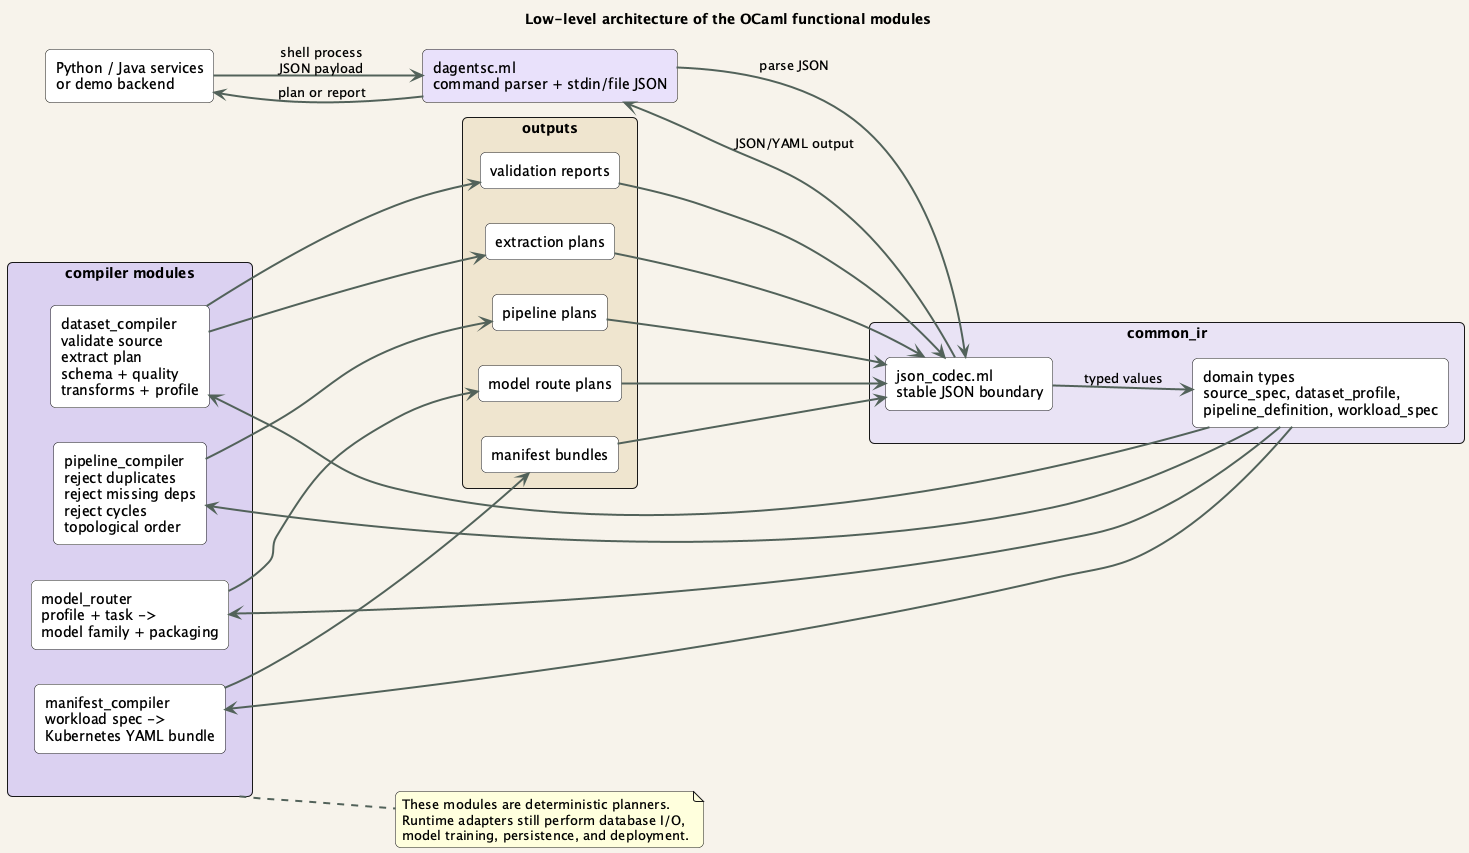
\includegraphics[width=\textwidth]{../presentation/puml/ocaml_module_architecture.png}
\caption{Low-level architecture of the OCaml functional modules.}
\label{fig:ocamlmodules}
\end{figure*}

The modules are:

\begin{itemize}
  \item \texttt{common\_ir}: shared types for sources, records, profiles,
  pipelines, models, quality rules, transforms, and workloads.
  \item \texttt{dataset\_compiler}: schema inference, source validation,
  extraction planning, schema contract validation, quality checks, transform
  planning, and profile building.
  \item \texttt{pipeline\_compiler}: duplicate step checks, missing dependency
  checks, cycle checks, and topological ordering.
  \item \texttt{model\_router}: maps a dataset profile and task type to model
  candidates and a packaging mode.
  \item \texttt{manifest\_compiler}: converts workload specs into Kubernetes
  YAML bundles.
  \item \texttt{json\_codec}: stable JSON input and output for service calls.
  \item \texttt{dagentsc}: command-line entry point used by Python and Java
  services.
\end{itemize}

\subsection{Why OCaml Was Useful}

OCaml was useful because the planning logic has many closed choices. Examples
include source kinds, task types, model families, quality operators, pipeline
step kinds, and workload kinds. These are naturally represented with variant
types and records.

Pattern matching makes each decision visible. For example, when a new source
kind is added, the planner code has clear places that must be updated. Pure
functions also make tests easier because the same input always gives the same
output.

\subsection{When OCaml Runs}

The OCaml layer is used in two ways. First, it is built before the app runs.
Docker images compile and copy the \texttt{dagentsc} binary. Second, services
call \texttt{dagentsc} at request time for validation and planning.

\begin{figure}[t]
\centering
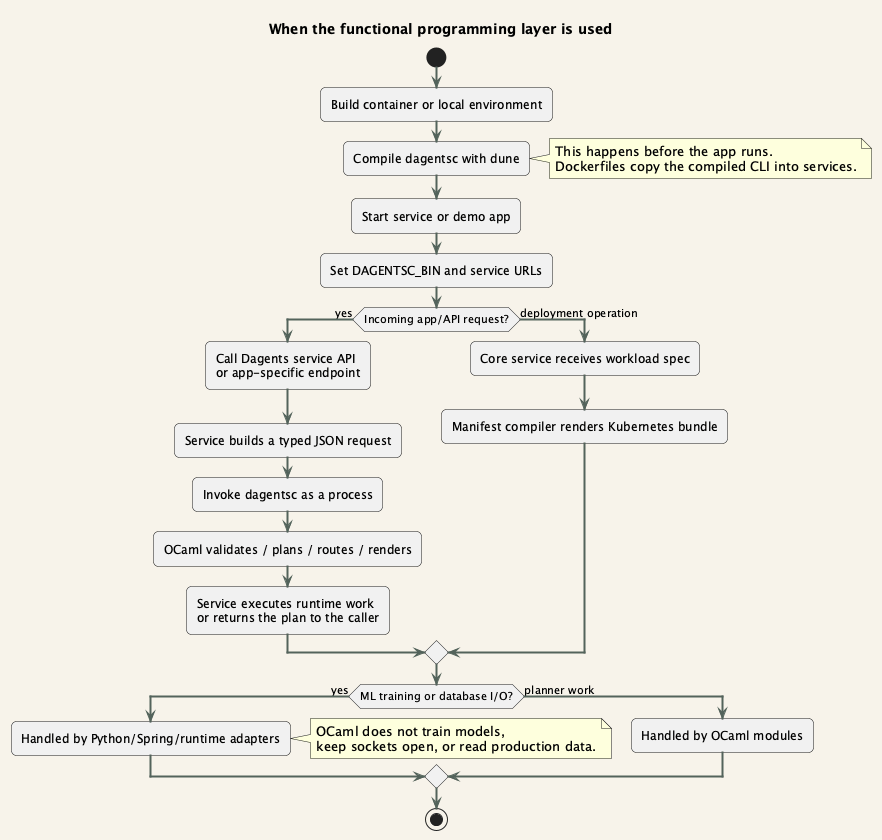
\includegraphics[width=\columnwidth]{../presentation/puml/ocaml_usage_timing.png}
\caption{When the functional programming layer is used.}
\label{fig:timing}
\end{figure}

OCaml does not train models, open database sockets, run a web server, or apply
Kubernetes manifests. Those actions stay in runtime services. OCaml returns the
plan that those services can execute.

\section{Core Functional Tasks}

Dagents supports several important planning tasks.

\subsection{Source Profiling}

Source profiling means reading the shape of a source and summarizing it before
model execution. For example, if a schema source contains records for
\texttt{table\_name}, \texttt{column\_name}, and \texttt{dtype}, the profiler
can return record count, feature fields, numeric fields, categorical fields,
partition count, and suggested model families.

\subsection{Pipeline Orchestration}

Pipeline orchestration means registering a workflow and running its steps in a
safe order. For example, a schema workflow can first attach the user question,
then profile schema records, then summarize columns, then project the context
needed for SQL generation. The pipeline planner rejects invalid graphs before
runtime.

\subsection{Model Routing}

Model routing chooses suitable model families for a task. For a text or
embedding task, Dagents can route toward transformer-style models. For tabular
anomaly detection, it can route toward autoencoders or random forests. The
router does not run the model. It decides what should be run.

\subsection{Manifest Generation}

Manifest generation converts a typed workload spec into Kubernetes YAML. For
example, the NL2SQL backend can be described as a Deployment with one HTTP
port, environment variables, resource limits, a Service, and a ConfigMap. The
manifest compiler turns that into a repeatable deployment bundle.

\subsection{Workloads and Workload Compilation}

A workload is the unit of runtime deployment. It can be a service, model job,
pipeline worker, or scheduled task. Workload compilation means taking a clean
Dagents workload spec and generating concrete deployment artifacts from it.
This makes deployment less dependent on hand-written YAML.

\section{Service API Example}

A backend can integrate with Dagents by calling service APIs and the
\texttt{dagentsc} planner. A simplified workload compile request is shown
below.

\begin{lstlisting}[style=dagents]
POST /api/v1/workloads:compile
{
  "plan_id": "nl2sql-demo",
  "namespace": "dagents-demo",
  "include_services": true,
  "include_config_maps": true,
  "components": [
    {
      "name": "nl2sql-demo-backend",
      "image": "dagents/nl2sql-demo-backend:local",
      "kind": "Deployment",
      "replicas": 1,
      "ports": [
        { "name": "http", "container_port": 8070 }
      ],
      "env": [
        { "name": "NL2SQL_DEFAULT_MODEL_ID",
          "value": "codet5p_spider_model" }
      ]
    }
  ]
}
\end{lstlisting}

The core service returns a workload plan with rendered manifests. The backend
does not need to manually write every Kubernetes object.

\section{NL2SQL Quick Demo}

The NL2SQL quick demo is located under \texttt{services/nl2sql-demo}. It has a
React frontend and a FastAPI backend. The user selects or edits a schema,
enters a natural-language question, selects a model adapter, and generates SQL.

\begin{figure*}[t]
\centering
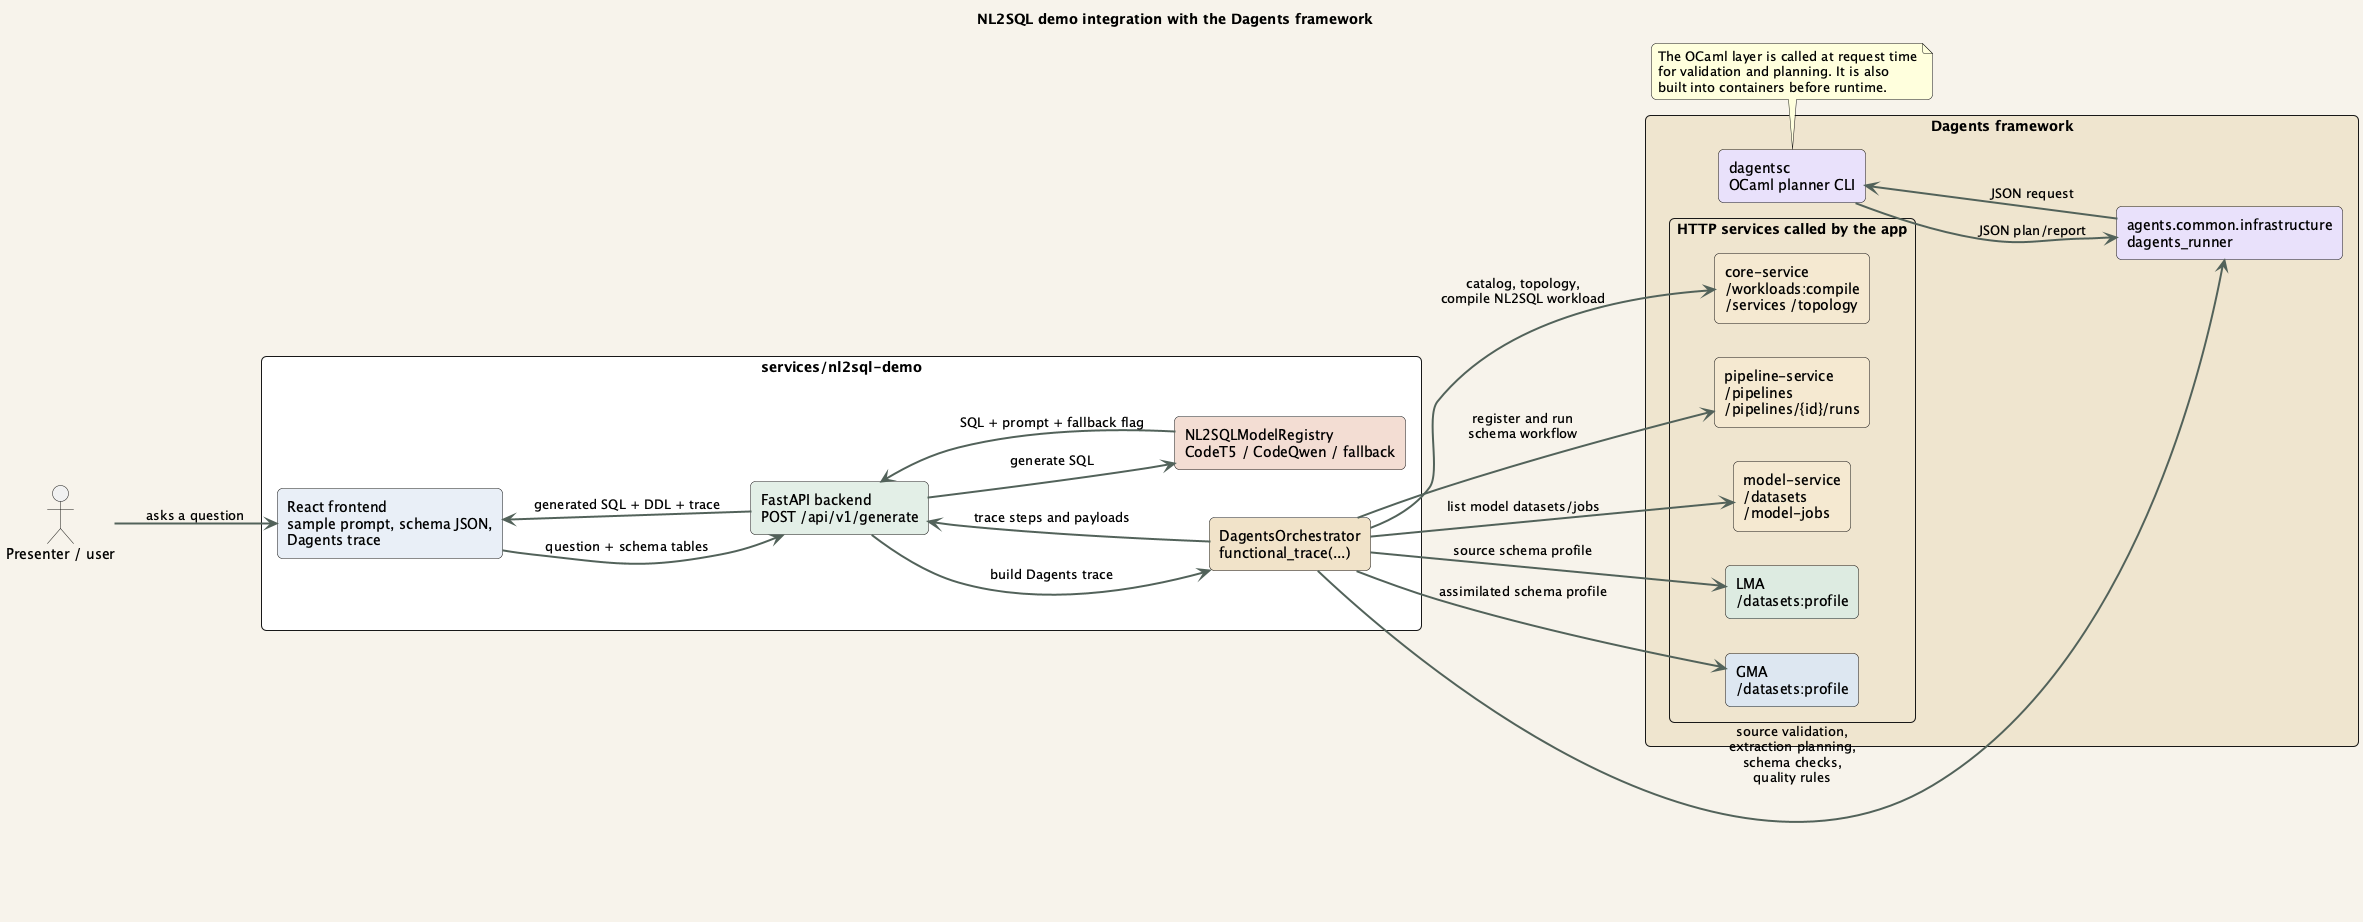
\includegraphics[width=\textwidth]{../presentation/puml/nl2sql_dagents_integration.png}
\caption{NL2SQL quick demo integration with the Dagents framework.}
\label{fig:nl2sql}
\end{figure*}

The backend performs three jobs:

\begin{itemize}
  \item builds DDL context from the schema tables;
  \item calls the selected NL2SQL model adapter or deterministic fallback;
  \item builds a Dagents trace using planners and services.
\end{itemize}

The trace includes:

\begin{itemize}
  \item SourceSpec validation;
  \item extraction planning;
  \item schema contract validation;
  \item data quality checks;
  \item pipeline DAG planning;
  \item model route planning;
  \item core-service catalog, topology, and workload compilation;
  \item pipeline-service registration and run execution;
  \item model-service catalog and recent job access;
  \item LMA source registration, validation, profiling, and source model job;
  \item GMA registration, heartbeat, source validation, aggregate profiling,
  aggregate model job, deployment sync, run dispatch, and fleet overview.
\end{itemize}

This answers an important design question: NL2SQL does use LMA and GMA in the
Dagents sense. The LMA side handles source-scoped schema work. The GMA side
handles aggregate coordination and multi-source style work. The demo also
registers the NL2SQL LMA with GMA and sends a heartbeat.

\subsection{Model Adapters and Fallback}

The demo supports CodeT5-style and CodeQwen LoRA-style artifacts from the
notebooks. These artifacts are loaded lazily from zip files under
\texttt{models/}. For presentation safety, the app also has a deterministic
fallback adapter. The fallback is useful when a GPU, model dependency, or
artifact path is unavailable.

The backend now returns a \texttt{fallback\_detail} field. This makes failures
clear. Instead of only saying that fallback was used, the app can show whether
the real cause was an import error, missing model config, or hardware/runtime
issue.

\section{Current Project State}

At the final stage, the project contains:

\begin{itemize}
  \item working OCaml planner modules under \texttt{bindings/ocaml};
  \item a \texttt{dagentsc} CLI for JSON-based planner calls;
  \item LMA and GMA FastAPI services;
  \item core-service, pipeline-service, and model-service;
  \item Dockerfiles and Docker Compose wiring;
  \item Spring service variants for core/control paths;
  \item demo scripts under \texttt{docs/demo} and \texttt{services/nl2sql-demo/scripts};
  \item PUML architecture diagrams and rendered images;
  \item NL2SQL quick demo with model adapters and a visible Dagents trace.
\end{itemize}

The main implemented APIs include:

\begin{itemize}
  \item \texttt{GET /api/v1/health};
  \item \texttt{GET /api/v1/services};
  \item \texttt{GET /api/v1/topology};
  \item \texttt{POST /api/v1/workloads:compile};
  \item \texttt{POST /api/v1/pipelines};
  \item \texttt{POST /api/v1/pipelines/\{id\}/runs};
  \item \texttt{POST /api/v1/datasets:profile};
  \item \texttt{POST /api/v1/model-jobs};
  \item \texttt{PUT /api/v1/agents/\{id\}/registration};
  \item \texttt{POST /api/v1/agents/\{id\}/heartbeats};
  \item \texttt{POST /api/v1/generate} for the NL2SQL quick demo.
\end{itemize}

\section{Testing and Verification}

The OCaml layer is tested with Dune. The tests cover schema inference, source
validation, extraction planning, partition planning, schema contract checks,
quality reports, transforms, pipeline ordering, cycle rejection, model routing,
manifest rendering, and JSON codec round trips.

\begin{lstlisting}[style=dagents]
cd bindings/ocaml
opam exec -- dune test
\end{lstlisting}

The NL2SQL backend tests verify health, samples, model descriptors, SQL
generation, fallback metadata, and the expanded LMA/GMA trace.

\begin{lstlisting}[style=dagents]
python -m unittest services/nl2sql-demo/tests/test_nl2sql_api.py
\end{lstlisting}

The frontend build also passed:

\begin{lstlisting}[style=dagents]
cd services/nl2sql-demo/frontend
npm run build
\end{lstlisting}

Docker Compose configuration validates when the env file is supplied:

\begin{lstlisting}[style=dagents]
docker compose --env-file env/.env.compose config --quiet
\end{lstlisting}

The run scripts now check whether Docker Desktop is running and fail with a
clear message if the daemon is unavailable.

\section{Design Tradeoffs}

\subsection{Why Not Put Everything in OCaml?}

The project keeps ML training, HTTP APIs, database access, and deployment
execution outside OCaml. Python and Java are better suited for those parts
because they have strong service and ML ecosystems. OCaml is used only where it
adds clear value: typed planning and deterministic transformation.

\subsection{Why Use a Process Boundary?}

The project uses \texttt{dagentsc} as a subprocess instead of direct FFI. This
keeps the boundary simple. Services can pass JSON in, receive JSON out, and
handle planner failure without crashing the service process.

\subsection{Why Keep a Deterministic NL2SQL Fallback?}

The fallback keeps the demo usable even when model artifacts, GPU memory, or
optional ML dependencies are unavailable. It is not a replacement for the real
model adapters. It is a presentation-safe path that still shows the Dagents
trace and service integration.

\section{Limitations and Future Work}

The main limitations are:

\begin{itemize}
  \item persistence is still mostly in-memory for several services;
  \item broker-backed messaging is not fully integrated;
  \item production source connectors need more hardening;
  \item NL2SQL model quality depends on artifact quality and runtime resources;
  \item the OCaml planner currently communicates through JSON subprocess calls,
  which is simple but not the fastest possible boundary.
\end{itemize}

Future work should add durable stores, broker-backed communication, stronger
source adapters, CI-based container runs, and more model families. The OCaml
layer can also grow with additional typed planners as Dagents adds more
workload kinds.

\section{Work Distribution}

The work was split around system and functional responsibilities:

\begin{itemize}
  \item \textbf{Pradyun Devarakonda}: OCaml functional modules, planner CLI,
  dataset/pipeline/model/manifest planning, NL2SQL backend orchestration, demo
  scripts, and report material.
  \item \textbf{Dheeraj Rajanala}: service architecture support, LMA/GMA flow
  validation, NL2SQL model artifact work, frontend/demo support, and testing
  support.
\end{itemize}

Both members contributed to integration, debugging, presentation material, and
final verification.

\section{Conclusion}

Dagents shows how functional programming can be used inside a real service
architecture without replacing the whole stack. OCaml provides a typed planner
kernel. Python and Java services provide runtime execution and integration.
LMA and GMA provide local and global agent boundaries. The NL2SQL quick demo
shows how a downstream application can use the same framework for validation,
planning, routing, service orchestration, and traceability.

The main result is a working framework that is easier to explain than a set of
ad hoc services. Inputs become typed plans. Plans are tested. Services execute
them. That separation is the central value of the project.

\begin{thebibliography}{1}

\bibitem{milner}
R. Milner, ``A theory of type polymorphism in programming,'' \emph{Journal of
Computer and System Sciences}, vol. 17, no. 3, pp. 348--375, 1978.

\bibitem{ocaml}
X. Leroy, D. Doligez, A. Frisch, J. Garrigue, D. Remy, and J. Vouillon,
\emph{The OCaml System: Documentation and User's Manual}. OCaml.org. [Online].
Available: \url{https://ocaml.org/manual/}

\bibitem{t5}
C. Raffel et al., ``Exploring the limits of transfer learning with a unified
text-to-text transformer,'' \emph{Journal of Machine Learning Research},
vol. 21, no. 140, pp. 1--67, 2020.

\bibitem{codet5}
Y. Wang, W. Wang, S. R. Joty, and S. C. H. Hoi, ``CodeT5:
Identifier-aware unified pre-trained encoder-decoder models for code
understanding and generation,'' in \emph{Proc. EMNLP}, 2021.

\bibitem{spider}
T. Yu et al., ``Spider: A large-scale human-labeled dataset for complex and
cross-domain semantic parsing and text-to-SQL task,'' in \emph{Proc. EMNLP},
2018.

\bibitem{lora}
E. Hu et al., ``LoRA: Low-rank adaptation of large language models,'' in
\emph{Proc. ICLR}, 2022.

\bibitem{kubernetes}
The Kubernetes Authors, ``Workloads,'' Kubernetes Documentation. [Online].
Available: \url{https://kubernetes.io/docs/concepts/workloads/}

\end{thebibliography}

\end{document}
